\begin{comment}
\documentclass[11pt]{article}  % , titlepage
\usepackage{Common/toshi}
\begin{document}
\end{comment}



%%%%%%%%%%%%%%%%%% section 1 %%%%%%%%%%%%%%%%%%%%%%%%%%%%%%%%%
\section{Introduction}
\label{sec:intro}


Over the past decades, gauge theories have been one of the most
important subjects in theoretical physics.
They describe the fundamental interaction among elementary particles
and are building blocks of the standard model of particle physics.
Still, however, the non-perturbative dynamics of quantum gauge theories
has not been fully uncovered.

A breakthrough was initiated by the discovery of exact solutions to
the low energy effective action of certain $\CN=2$ supersymmetric gauge
theories in the pioneering works by Seiberg and Witten \cite{Seiberg:1994rs,Seiberg:1994aj}.
In their work, a Riemann surface and a differential on it, today such a pair is referred to as
``Seiberg-Witten curve'' and ``Seiberg-Witten differential,'' played a significant role, and it brought to us
rich connections to two-dimensional integrable systems \cite{Gorsky:1995zq,Martinec:1995by,Donagi:1995cf,Itoyama:1995nv}.
It was also the first time that the techniques in algebraic geometry were introduced
to theoretical physics.

The work of Seiberg and Witten was based on certain assumptions on the strong coupling
behavior of the relevant gauge theories, but it was somewhat heuristic.
Then, it was a great progress when it was shown that the mathematical description for
the prepotential conjectured by Seiberg and Witten can be obtained by an honest
calculation of the quantum corrections to a certain two-parameter
deformation of the prepotential to all orders in the instanton
expansion \cite{Nekrasov:2002qd,Nekrasov:2003rj,Nakajima:2003pg}.

Soon after these prominent works, there were two more major developments in the study of
supersymmetric gauge theories.
First, Pestun reformulated the method of supersymmetric localization \cite{Pestun:2007rz},
which generalizes previous works and allows us to exactly compute partition functions
and a class of observables for supersymmetric gauge theories on $S^4$.
Based on Pestun's result, another progress was achieved by
Alday, Gaiotto and Tachikawa \cite{Alday:2009aq}, which
is now well known as AGT correspondence.
The AGT correspondence relates four-dimensional supersymmetric gauge theories on $S^4$ and
two-dimensional (non-supersymmetric) Liouville/Toda conformal field theory.
Not only did it provide new interesting dualities among quantum field theories,
but also has promoted fruitful interactions between physicists and mathematicians.
%Involving these progresses, supersymmetric gauge theories have provide us
%many more interesting \emph{exact results}.
These interesting phenomena, involving the work of Seiberg and Witten,
can naturally be understood from the string theory viewpoint \cite{Witten:1997sc,Gaiotto:2009we}.
In addition, the techniques to compute exact physical quantities provide us many nontrivial checks
for AGT correspondence, AdS/CFT correspondence,
and other dualities in quantum field theories such as S-duality.


Behind the ``exact solvability'' of supersymmtric gauge theories, generically there are certain integrable
structures, as in Seiberg-Witten curve, and they play a crucial role for the gauge theories to be
exactly solvable.
In fact, it is suggested that the AGT correspondence and many related developments can ultimately
be understood as consequences of the integrable structure in
supersymmetric field theories \cite{Gaiotto:2009hg,Teschner:2010je}.
In some cases concrete correspondences between
supersymmetric gauge theory and integrable system were established and investigated,
e.g.~\cite{Nekrasov:2009uh,Nekrasov:2009ui,Nekrasov:2009rc,Nekrasov:2010ka,Nekrasov:2011bc,Yamazaki:2012cp,Terashima:2012cx,Yamazaki:2013nra,Nekrasov:2015wsu}.
Then, we come up with two questions:
\begin{itemize}
    \item Why is there an integrable system behind supersymmetric gauge theory?
    \item Why, at all, does integrable system exist?
\end{itemize}
The second question might look fancy, but we will explain its meaning in a moment.
It turns out that these two questions are really addressed into a single answer:
it is because there is a \emph{topological} quantum field theory
equipped with line operators localized in extra dimensions.
This statement is to be the main theme of this thesis, but let us pause here and
%give an introductory review
begin with a brief introduction
to integrable system.


Integrable system, or integrable model,%
%
\footnote{Throughout this thesis, we will use the terms \emph{integrable system} and
\emph{integrable model} interchangeably.}
%
may have several definitions (or characterizations),
but a canonical one should be the \emph{Yang-Baxter equation} with \emph{spectral parameters},
that is graphically represented by
\begin{equation}
    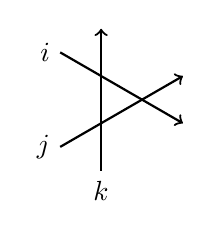
\begin{tikzpicture}[scale=0.6, baseline=(x.base)]
        \node (x) at (30:2) {};

        \draw[thick, ->] (0,0) node[left] {$j$} -- ++(30:3);
        \draw[thick, ->] (0,2) node[left] {$i$} -- ++(-30:3);
        \draw[thick, ->] (-30:1) node[below] {$k$} -- ++(0,3);

    \end{tikzpicture}
  \ =
    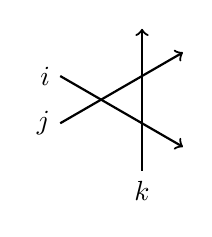
\begin{tikzpicture}[scale=0.6, baseline=(x.base)]
        \node (x) at (30:1) {};

        \draw[thick, ->] (0,0) node[left] {$j$} -- ++(30:3);
        \draw[thick, ->] (0,1) node[left] {$i$} -- ++(-30:3);
        \draw[thick, ->] (-30:2) node[below] {$k$} -- ++(0,3);

    \end{tikzpicture}
    \quad ,
\label{eq:intro_ybe0}
\end{equation}
where three intersecting lines are called \emph{rapidity lines} in the literature.
Each rapidity line carries a set of a vector space $V$ and a spectral parameter $u$
taking values in a Riemann surface.
At each crossing of the two lines, say $i$ and $j$, we associate an \emph{R-matrix}:
\begin{equation}
    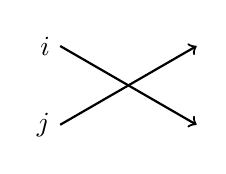
\begin{tikzpicture}[scale=1, baseline=(x.base)]  \node (x) at (0,0) {\vphantom{x}};

        \draw[thick, ->] (0,-0.5) node[left] {$j$} -- ++(30:2);
        \draw[thick, ->] (0,0.5) node[left] {$i$} -- ++(-30:2);

    \end{tikzpicture}
    \ =: \
    R_{ij}(u_i,u_j) \in \End(V_i\otimes V_j).
\end{equation}
Then, the Yang-Baxter equation reads
\begin{equation}
    R_{ij}(u_{i},u_{j})R_{ik}(u_{i},u_{k})R_{jk}(u_{j},u_{k})
        =  R_{jk}(u_{j},u_{k})R_{ik}(u_{i},u_{k})R_{ij}(u_{i},u_{j})
        ,
    \label{eq:intro_ybe}
\end{equation}
where each R-matrix is extended to an operator
$R_{ij}:=R_{ij}\otimes {\rm id}_{V_k}\in\End(V_i\otimes V_j\otimes V_k)$, etc.
R-matrix satisfying the Yang-Baxter equation implies a global relation,
that is, the transfer matrices constructed from the R-matrices commute each other.
When we have commuting transfer matrices, by expanding them with respect to the spectral parameters,
we obtain an infinite number of commuting conserved charges, that is another
definition of integrability.


Once we have the Yang-Baxter equation, we solve it and the solution yields an
integrable model.
This is, however, highly nontrivial.
For example, if one naively tries to solve the Yang-Baxter equation \eqref{eq:intro_ybe},
one finds that these equations are over-constrained in general.
To see this, let all the vector spaces $V_i$ be $N$-dimensional for simplicity.
Then the R-matrix associated with each crossing has four boundary lines and hence
has $O(N^4)$ components.
On the other hand, the Yang-Baxter equation, associated with diagrams with six boundary lines,
has $O(N^6)$ equations.
Even if one considers the simplest nontrivial case, $N=2$, the R-matrix has $16$ components
while they are constrained by $64$ equations.
The larger $N$ becomes, the severer this over-counting problem gets.
Thus, at first sight it seems hopeless that we could have a solution to the Yang-Baxter equation
\eqref{eq:intro_ybe},
but we know there exist solutions as well.


Now we arrive at the question: why integrable model exists?
If we have a good understanding of this question, then we can try to understand existing
integrable models from a unified perspective.
Furthermore, we may try to find new integrable models based on such understanding.
%
Indeed, there are two approaches to this question, both based on the ideas from quantum
field theory.
%For both approaches, the key concept is that there is a topological quantum field theory
%equipped with line operators localized in an extra dimensions.
%Actually,
These two approaches can also provide an answer to the first question given above.
Let us introduce them in order.


The first approach is based on four-dimensional analogue of Chern-Simons theory,
which is a cousin of the usual three-dimensional Chern-Simons theory but somewhat exotic.
The four-dimensional Chern-Simons theory can be defined only on a product manifold of a two-dimensional plane
and a Riemann surface, and the theory is partially topological and partially holomorphic on each two-manifold.
%they showed that the line operators extending
This theory was pioneered by Costello \cite{Costello:2013zra,Costello:2013sla},
and further investigated in \cite{Witten:2016spx,Costello:2017dso,Costello:2018gyb,Costello:2019tri}.
The ordinary three-dimensional Chern-Simons theory produces
quantum invariants of knots, links, and three-manifolds \cite{Witten:1988hf}.
It is well known that knots and links are closely related to integrable systems
(see e.g.~\cite{Wadati:1989ud} and the references therein),
but a direct connection between Chern-Simons theory and integrable systems was missing.
Costello, Witten and Yamazaki showed that in four-dimensional Chern-Simons theory, line operators
extending the topological plane generate a lattice model, and it is really an integrable lattice model.
An important fact here is that the line operators can be elongated only in the topological plane,
and their coordinates localized at the Riemann surface play the role of spectral parameters.
Therefore, what they demonstrated is that an integrable lattice model comes from line operators in a topological
quantum field theory with extra dimensions.


Another approach is based on supersymmetric quiver gauge theories, which is our main focus in this thesis.
Today this approach is called \emph{Gauge/YBE correspondence} \cite{Yamazaki:2012cp,Terashima:2012cx,Yamazaki:2013nra}.
This correspondence claims a more direct relation between the partition function, or supersymmetric index,
of quiver gauge theories and the partition function of integrable lattice models.
In fact, in this correspondence there is one-by-one mapping
between quiver gauge theories and integrable lattice models,
such as an identification between the quiver diagram and the lattice of an integrable spin system;
see figure \ref{fig:intro_gauge_ybe}.%
%
\footnote{More specifically, the index for vector and chiral multiplets
in quiver gauge theories are identified with the Boltzmann weights for
self- and nearest-neighbor interaction of spin systems, respectively.
We will show an explicit dictionary in section \ref{sec:tiling_latticemodel} of the main text.}
%
%
%FIGURE
\begin{figure}
    \centering
      \subfloat[\label{}]{
        \begin{tikzpicture}[scale=0.8, baseline=(x.base)]  \node (x) at (0,0) {\vphantom{x}};
          \def\site{1.2cm}

          \node[gnode] (a1) at (0,0) {};\node[gnode] (a2) at (\site,0) {};\node[gnode] (a3) at (2*\site,0) {};\node[gnode] (a4) at (3*\site,0) {};
          \begin{scope}[yshift=\site]
          \node[gnode] (b1) at (0,0) {};\node[gnode] (b2) at (\site,0) {};\node[gnode] (b3) at (2*\site,0) {};\node[gnode] (b4) at (3*\site,0) {};
          \end{scope}
          \begin{scope}[yshift=2*\site]
          \node[gnode] (c1) at (0,0) {};\node[gnode] (c2) at (\site,0) {};\node[gnode] (c3) at (2*\site,0) {};\node[gnode] (c4) at (3*\site,0) {};
          \end{scope}

          \draw[semithick, arrows=-latex] (a1) to (a2);\draw[semithick, arrows=-latex] (a3) to (a2);\draw[semithick, arrows=-latex] (a3) to (a4);
          \draw[semithick, arrows=-latex] (b2) to (b1);\draw[semithick, arrows=-latex] (b2) to (b3);\draw[semithick, arrows=-latex] (b4) to (b3);
          \draw[semithick, arrows=-latex] (c1) to (c2);\draw[semithick, arrows=-latex] (c3) to (c2);\draw[semithick, arrows=-latex] (c3) to (c4);

          \draw[semithick, arrows=-latex] (b1) to (a1);\draw[semithick, arrows=-latex] (a2) to (b2);
          \draw[semithick, arrows=-latex] (b3) to (a3);\draw[semithick, arrows=-latex] (a4) to (b4);
          \draw[semithick, arrows=-latex] (b1) to (c1);\draw[semithick, arrows=-latex] (c2) to (b2);
          \draw[semithick, arrows=-latex] (b3) to (c3);\draw[semithick, arrows=-latex] (c4) to (b4);

          \draw[semithick] (a1) to ++(-\site/2,0);\draw[semithick, arrows=latex-] (b1) to ++(-\site/2,0);\draw[semithick] (c1) to ++(-\site/2,0);
          \draw[semithick, arrows=latex-] (a4) to ++(\site/2,0); \draw[semithick] (b4) to ++(\site/2,0); \draw[semithick, arrows=latex-] (c4) to ++(\site/2,0);

          \draw[semithick, arrows=latex-] (a1) to ++(0,-\site/2);\draw[semithick] (a2) to ++(0,-\site/2);
          \draw[semithick, arrows=latex-] (a3) to ++(0,-\site/2);\draw[semithick] (a4) to ++(0,-\site/2);
          \draw[semithick, arrows=latex-] (c1) to ++(0,\site/2); \draw[semithick] (c2) to ++(0,\site/2);
          \draw[semithick, arrows=latex-] (c3) to ++(0,\site/2); \draw[semithick] (c4) to ++(0,\site/2);

        \end{tikzpicture}
        }
    \qquad\qquad
      \subfloat[\label{}]{
        \begin{tikzpicture}[scale=0.8, baseline=(x.base)]  \node (x) at (0,0) {\vphantom{x}};
          \def\site{1.2cm}

          \draw[semithick] (0,-\site/2) -- ++(0,3*\site);
          \draw[semithick, xshift=\site] (0,-\site/2) -- ++(0,3*\site);
          \draw[semithick, xshift=2*\site] (0,-\site/2) -- ++(0,3*\site);
          \draw[semithick, xshift=3*\site] (0,-\site/2) -- ++(0,3*\site);

          \draw[semithick] (-\site/2,0) -- ++(4*\site,0);
          \draw[semithick, yshift=\site] (-\site/2,0) -- ++(4*\site,0);
          \draw[semithick, yshift=2*\site] (-\site/2,0) -- ++(4*\site,0);

          \node[spin] (a1) at (0,0) {$s$};\node[spin] (a2) at (\site,0) {$s$};
          \node[spin] (a3) at (2*\site,0) {$s$};\node[spin] (a4) at (3*\site,0) {$s$};
          \begin{scope}[yshift=\site]
          \node[spin] (b1) at (0,0) {$s$};\node[spin] (b2) at (\site,0) {$s$};
          \node[spin] (b3) at (2*\site,0) {$s$};\node[spin] (b4) at (3*\site,0) {$s$};
          \end{scope}
          \begin{scope}[yshift=2*\site]
          \node[spin] (c1) at (0,0) {$s$};\node[spin] (c2) at (\site,0) {$s$};
          \node[spin] (c3) at (2*\site,0) {$s$};\node[spin] (c4) at (3*\site,0) {$s$};
          \end{scope}


        \end{tikzpicture}
        }
      \caption{In the Gauge/YBE correspondence, the quiver diagram specifying a
      gauge theory is identified with the lattice of an integrable spin system.}
      \label{fig:intro_gauge_ybe}
    \end{figure}
%
%
A topological structure behind the Gauge/YBE correspondence was elucidated in \cite{Yagi:2015lha}.
It is again a topological quantum field theory equipped with line operators
localized in extra dimensions.


Actually, four-dimensional Chern-Simons theory can eventually be
embedded into string theory setup \cite{Costello:2018txb} and
both approaches above are related to each other.
Based on these observations, we may conclude that the answer to the question
``why is there an integrable system behind supersymmetric gauge theory'' is
that we have a topological quantum field theory with line operators.
Moreover, this also answers to the question ``why does integrable system exist,''
since it is manifest that the Yang-Baxter equation \eqref{eq:intro_ybe0} is
satisfied by the topological nature of the system. %line operators in a topological quantum field theory
(Here notice that rapidity lines shown in \eqref{eq:intro_ybe0} are viewed as
line operators in a topological quantum field theory.)


The aim of this thesis is to give a unified picture of the above two approaches
using branes in string theory,
and present a more elaborate description of the correspondence between
supersymmetric gauge theories and integrable lattice models.
In doing so, we proceed to introducing further defect operators in
supersymmetric gauge theories. Then we can study its counterpart in integrable
lattice model side.
Our main result in \cite{Maruyoshi:2020cwy} is that a brane realization of the correspondence connects
three objects in different areas:
transfer matrices in trigonometric quantum integrable systems,
Wilson-'t Hooft lines in four-dimensional quiver gauge theories on $S^1\times \R^3$, and
Verlinde line operators in two-dimensional Liouville/Toda conformal field theory.
Furthermore, we also clarify such a correspondence among the three is naturally understood
from the perspective of four-dimensional Chern-Simons theory through string dualities.


We show that the introduction of such additional defects enriches our correspondence,
and hopefully provide an insight into a new integrable system.
We will mostly work in the second approach, namely the correspondence between
quiver gauge theory and integrable lattice model.
%Both of our approach and that of four-dimensional Chern-Simons theory can eventually be
%embedded into string theory setup \cite{Costello:2018txb}.
%The both approaches are eventually embedded into string theory setup \cite{Costello:2018txb}.
We finally make comments on how our formulation of the correspondence is related to the setup of
four-dimensional Chern-Simons theory
%and clarify the relationship between the two
from the view point of brane realization and string dualities.
%four-dimensional Chern-Simons theory
%and our construction of the correspondences.







\subsection*{Organization of the thesis}


%FIGURE
\begin{figure}
    \centering
        %\subfloat[\label{}]{  }
        %\subfloat[\label{}]{  }
        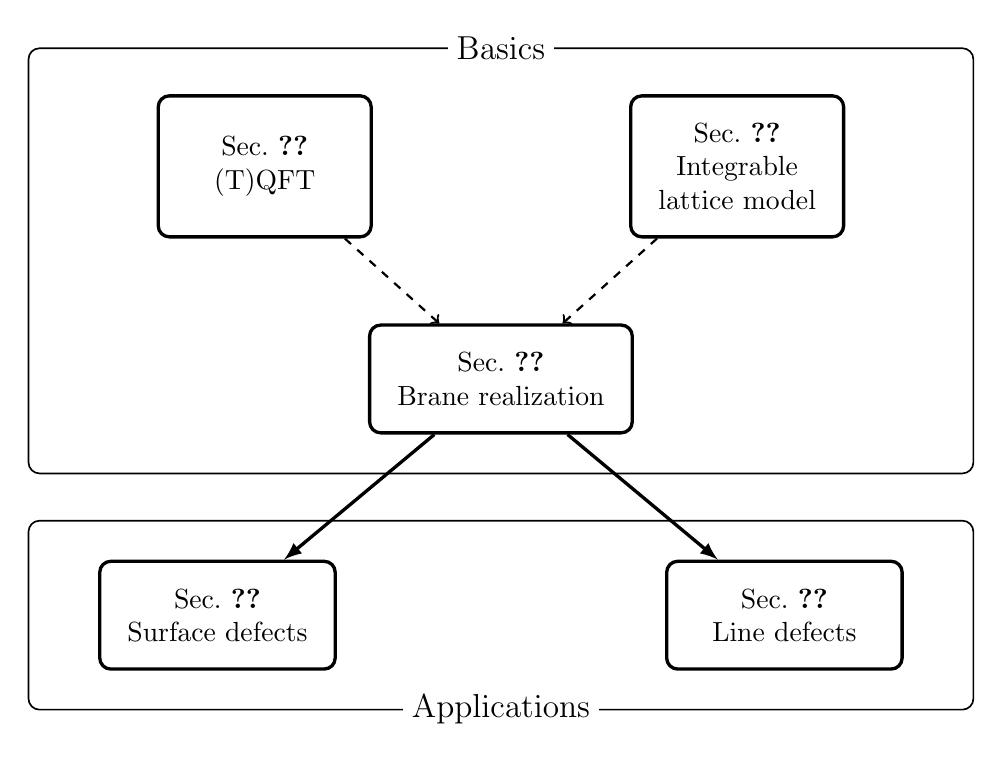
\begin{tikzpicture}[scale=1, baseline=(x.base), font=\normalsize]  \node (x) at (0,0) {\vphantom{x}};
            \def\sep{3cm}
            \tikzset{mysec/.style={rectangle,rounded corners,draw=black, %top color=white, bottom color=yellow!50,
                very thick, inner sep=1em, minimum size=3em, text centered}}

        \node[mysec, align=center] (B) at (0,0) {Sec.~\ref{sec:integrability_from_TQFT} \\ Brane realization};
        \node[mysec, align=center] (I) at (\sep,0.9*\sep) {Sec.~\ref{sec:lattice_model} \\ Integrable \\ lattice model};
        \node[mysec, align=center, text opacity=0] (T) at (-\sep,0.9*\sep) {Sec.~\ref{sec:lattice_model} \\ Integrable \\ lattice model};
        \node[align=center] at (-\sep,0.9*\sep) {Sec.~\ref{sec:preliminaries} \\ (T)QFT};

        \node[mysec, align=center] (S) at (-1.2*\sep,-1*\sep) {Sec.~\ref{sec:surface} \\ Surface defects};
        \node[mysec, align=center, text opacity=0] (L) at (1.2*\sep,-1*\sep) {Sec.~\ref{sec:line} \\ Surface defects};
        \node[align=center] at (1.2*\sep,-1*\sep) {Sec.~\ref{sec:line} \\ Line defects};

        \draw[thick, dashed, arrows=-to] (T) to (B);
        \draw[thick, dashed, arrows=-to] (I) to (B);
        \draw[very thick, arrows=-latex] (B) to (S);
        \draw[very thick, arrows=-latex] (B) to (L);


        \draw[semithick, rounded corners] (-2*\sep,-0.6*\sep) rectangle (2*\sep,-1.4*\sep);
        \draw[semithick, rounded corners] (-2*\sep,-0.4*\sep) rectangle (2*\sep,1.4*\sep);

        \node[fill=white, text centered, font=\large] at (0,1.4*\sep) {Basics};
        \node[fill=white, text centered, font=\large] at (0,-1.4*\sep) {Applications};


        \end{tikzpicture}
    \caption{Structure of the thesis.}
    \label{fig:structure}
\end{figure}


The structure of the thesis is shown as in figure \ref{fig:structure}.
Section \ref{sec:integrability} is devoted to a collection of basic facts regarding
topological quantum field theory, integrable lattice model, and
their realization by brane construction in string theory.
In section \ref{sec:preliminaries}, we briefly review the natural requirements for quantum field theory
and introduce Atiyah's axioms of topological quantum field theory (TQFT). Then we introduce lattice model as
a discrete version of quantum field theory in section \ref{sec:lattice_model}.
With these preparations, in section \ref{sec:integrability_from_TQFT}
we show that line operators in a topological quantum field theory and
integrable lattice models turn out to be equivalent through branes in string theory.
In section \ref{sec:surface}, we get into a concrete setup of the correspondence
between quiver gauge theories on spacetime $S^1\times S^3$ and
integrable lattice models of elliptic type.
There we add on additional surface defects in gauge theory side, and verify that they are
identified with the transfer matrix of the corresponding integrable lattice model.
In section \ref{sec:line}, we consider line defects in circular and linear quiver gauge
theories on $S^1\times \R^3$, which is based on the author's work \cite{Maruyoshi:2020cwy}.
Such line defects are represented as half-BPS Wilson-'t Hooft lines in gauge theories and
identified with transfer matrices of trigonometric type.
A variant of the AGT correspondence further implies an identification of the transfer matrices with
Verlinde line operators in Toda conformal field theory, which we also verify.
We clarify in section \ref{sec:branes} how these field theory setups are
related to four-dimensional Chern-Simons theory via embedding into string theory and dualities.
We conclude the thesis with some future directions in section \ref{sec:discussion}.


We also hope this thesis would be a good introductory review to the beautiful
and fascinating but largely unexplored connections among branes, topological
quantum field theories, and integrable systems.



%YBE can be seen as particle scattering and crossing of lattices













%%%%%%%%%%%%%%%%%%%%%%%%%%%%%%%%%%%%%%%%%%%%%%%%%%%%%%%%%



\bibliographystyle{Common/utphys}
%\nocite{*}
\bibliography{Common/Ref}



\end{document}